%% 
%% Copyright 2019-2024 Elsevier Ltd
%% 
%% This file is part of the 'CAS Bundle'.
%% --------------------------------------
%% 
\documentclass[a4paper,fleqn]{cas-sc}

\usepackage{amsmath,amssymb,amsfonts}
\usepackage{graphicx}
\usepackage{booktabs}
\usepackage{multirow}
\usepackage{array}
\usepackage{url}
\usepackage{xspace}

\usepackage[authoryear]{natbib}

%%% Author macros
\def\tsc#1{\csdef{#1}{\textsc{\lowercase{#1}}\xspace}}
\tsc{WGM}
\tsc{QE}


\begin{document}
\let\WriteBookmarks\relax
\def\floatpagepagefraction{1}
\def\textpagefraction{.001}

% Short title & Short authors for page headers
\shorttitle{2.5D Terrain Dataset Generation from RELLIS-3D \& Native 2.5D Path Planning Benchmark}
\shortauthors{Duc Anh et~al.}

% Main Title
\title [mode = title]{A Comprehensive Study on 2.5D Terrain Dataset Generation from RELLIS-3D and Benchmark Evaluation of Native 2.5D Autonomous Path Planning}

\tnotemark[1]
\tnotetext[1]{This technical report presents an end-to-end framework ranging from raw 3D LiDAR point cloud preprocessing into 2.5D digital elevation maps to experimental benchmarking of native 2.5D path planning algorithms for off-road autonomous ground vehicles.}

% Authors & Affiliations
\author[1]{Duc Anh}[orcid=0000-0002-1825-0097]
\cormark[1]
\fnmark[1]
\ead{ducanh.robotics@ptit.edu.vn}
\ead[url]{https://github.com/Whitenessly/Nhm1-2.5D}
\credit{Software, Methodology, Validation, Formal analysis, Writing - original draft}

\author[1]{Le Loc}
\fnmark[1]
\ead{leloc.robotics@ptit.edu.vn}
\credit{Data curation, Conceptualization, Investigation, Visualization}

\author[1]{Tue Lam}
\fnmark[1]
\ead{tuelam.robotics@ptit.edu.vn}
\credit{Conceptualization, Software, Validation, Writing - review and editing}

\affiliation[1]{organization={Faculty of Information Technology, Posts and Telecommunications Institute of Technology (PTIT)},
            addressline={Km 10, Nguyen Trai Road, Ha Dong District}, 
            city={Hanoi},
            postcode={100000}, 
            country={Vietnam}}

\cortext[1]{Corresponding author.}
\fntext[1]{Undergraduate researchers in Information Technology, Posts and Telecommunications Institute of Technology (PTIT).}

% Abstract
\begin{abstract}
Off-road autonomous navigation requires unmanned ground vehicles (UGVs) and legged robots to reliably perceive complex topography, navigate steep slopes, and accurately distinguish hazardous terrains such as mud pits, water puddles, and dense vegetation. This paper presents a complete, two-phase research and experimental pipeline:
\textbf{(1) 2.5D Multi-Layer Terrain Dataset Generation from RELLIS-3D:} We develop an automated processing pipeline that transforms raw 3D LiDAR point clouds (\texttt{.bin}) and semantic annotations (\texttt{.label}) into structured 2.5D grid representations stored in compressed \texttt{.npz} format, encompassing 25th-percentile digital elevation models (DEM), majority-voted semantic layers, spatial slope, surface roughness, traversability costmaps, and real-time visualization via ROS 2 RViz2.
\textbf{(2) Native 2.5D Kinodynamic Path Planning and Dataset Quality Benchmark:} We rigorously evaluate the fidelity and utility of our generated 2.5D representations across four state-of-the-art native 2.5D path planning algorithms: T-Hybrid A*, 2.5D RRT*, 2.5D Field D*, and 2.5D LazyPRM* (ArtPlanner).
Extensive benchmarking on $40.0\text{m} \times 30.0\text{m}$ complex terrain scenes ($0.2\text{m}$ resolution) demonstrates that 2.5D Field D* and 2.5D LazyPRM* achieve superior real-time execution speeds ($0.461\text{s} - 0.530\text{s}$), whereas T-Hybrid A* and 2.5D RRT* guarantee absolute chassis stability and zero rollover risk ($\bar{\tau} = 1.000, \text{Max Roll} = 0.00^\circ$). The proposed framework provides an effective and reproducible foundation for off-road robotics and digital terrain modeling.
\end{abstract}

% Keywords
\begin{keywords}
RELLIS-3D \sep Digital Elevation Model (DEM) \sep 2.5D Path Planning \sep Traversability Costmap \sep Semantic Terrain Analysis \sep Off-Road Navigation \sep ROS 2 RViz2
\end{keywords}

\maketitle

\section{Introduction}
\label{sec:intro}

Path planning is a fundamental capability that governs both the autonomy and operational safety of mobile robots. In structured indoor and urban environments, the operational surface is predominantly planar, allowing standard 2D occupancy grid maps to suffice. Conversely, in unstructured off-road environments—such as forests, agricultural fields, construction sites, and disaster search-and-rescue zones—robots continuously encounter severe undulations, steep embankments, mud pits, water bodies, dense thickets, and rugged rock formations \citep{pengjiang2020, jiayangliu2023, endo2024}.

Standard 2D flat representations discard vertical elevation and gradient profiles, preventing the vehicle from distinguishing between a gentle traversable slope and a precipitous cliff capable of causing a catastrophic rollover. On the other hand, full 3D point cloud or dense 3D voxel representations entail substantial memory footprints and high computational complexity, frequently surpassing the real-time processing capabilities of embedded onboard computers.

Consequently, the \textbf{2.5D Digital Elevation Model (2.5D DEM)} enriched with multi-layer geometric and semantic attributes emerges as the optimal compromise between fidelity and computational efficiency. This technical report presents a comprehensive, two-stage research and experimental framework:
\begin{enumerate}
    \item \textbf{Phase 1 -- 2.5D Dataset Generation from RELLIS-3D:} We design and implement an end-to-end software pipeline that ingests raw 3D LiDAR point clouds and semantic segmentations from the RELLIS-3D dataset, maps them into multi-attribute 2.5D grid representations (Elevation, Semantics, Slope, Roughness, Costmap, and Valid Mask) stored in \texttt{.npz} format, and validates them via ROS 2 RViz2.
    \item \textbf{Phase 2 -- Native 2.5D Trajectory Planning Benchmark \& Dataset Quality Validation:} We deploy and systematically benchmark four state-of-the-art native 2.5D planning algorithms (T-Hybrid A*, 2.5D RRT*, 2.5D Field D*, and 2.5D LazyPRM*) on the synthesized 2.5D terrain maps, assessing planning latency, 3D Euclidean path length, vehicle attitude stability (Roll/Pitch), and steep terrain traversability.
\end{enumerate}

\section{Overview of the RELLIS-3D Dataset}
\label{sec:rellis3d}

The RELLIS-3D dataset \citep{pengjiang2020} is a multimodal benchmark collected in unstructured off-road environments at the Rellis Campus of Texas A\&M University. It features synchronized RGB imagery, GPS/IMU inertial measurements, 64-beam Ouster OS1-64 LiDAR point clouds, and fine-grained point-wise semantic segmentation labels.

In this investigation, two primary data streams are utilized:
\begin{enumerate}
    \item \textbf{LiDAR Point Clouds in Binary Format (\texttt{.bin}):} Each reflected laser return $p_i$ is represented as a 4D feature vector:
    \begin{equation}
        p_i = (x_i, y_i, z_i, \text{intensity}_i)
    \end{equation}
    where $(x_i, y_i)$ denotes horizontal spatial coordinates, $z_i$ represents vertical elevation, and $\text{intensity}_i$ corresponds to the calibrated reflection intensity.
    \item \textbf{Semantic Annotation Labels (\texttt{.label}):} Each point contains a standard uint32 semantic class identifier denoting its physical terrain class or obstacle category (e.g., dirt, grass, tree, pole, water, mud, fence, bush, log).
\end{enumerate}

\section{2.5D Multi-Layer Terrain Dataset Generation Pipeline}
\label{sec:pipeline}

\subsection{Directory Structure and Output Data Components}
\label{subsec:components}
The processing pipeline ingests sequential LiDAR scans (\texttt{000000.bin}, \texttt{000001.bin}, \dots) along with their corresponding label files (\texttt{000000.label}, \texttt{000001.label}, \dots) and produces individual compressed \texttt{.npz} files in the target directory. Table \ref{tab:npz_components} summarizes the six core data layers encapsulated within each 2.5D map archive.

\begin{table}[width=\linewidth,cols=3,pos=htbp]
\caption{Core data layers extracted and stored in each 2.5D \texttt{.npz} map archive.}
\label{tab:npz_components}
\begin{tabular*}{\tblwidth}{@{} LLL@{} }
\toprule
\textbf{Component Layer} & \textbf{Data Type / Shape} & \textbf{Semantic Description \& Robotic Utility} \\
\midrule
\texttt{elevation}   & \texttt{float32} ($H \times W$) & 2.5D ground surface elevation model (meters). \\
\texttt{semantic}    & \texttt{uint32} ($H \times W$)  & Dominant semantic class determined via Majority Voting. \\
\texttt{slope}       & \texttt{float32} ($H \times W$) & Terrain inclination angle computed from elevation gradients (radians). \\
\texttt{roughness}   & \texttt{float32} ($H \times W$) & Local surface roughness derived from elevation standard deviation. \\
\texttt{costmap}     & \texttt{uint8} ($H \times W$)   & Fused traversability navigation costmap ($0 - 255$). \\
\texttt{valid\_mask} & \texttt{bool} ($H \times W$)    & Binary validity mask indicating cells populated with LiDAR points. \\
\bottomrule
\end{tabular*}
\end{table}

\subsection{Step 1: Point Cloud Extraction and Region of Interest (ROI) Filtering}
\label{subsec:step1_roi}
The point cloud data is loaded as \texttt{float32} tensors and reshaped into an $N \times 4$ array. Semantic labels are unpacked from raw 32-bit words using bitwise masking:
\begin{equation}
    \text{semantic\_id} = \text{label\_raw} \ \& \ \text{0xFFFF}
\end{equation}
To focus computational resources on the immediate traversable horizon and filter out distant ambient returns, the point cloud is bounded within a Region of Interest (ROI):
\begin{equation}
    x \in [x_{\min}, x_{\max}] = [-10.0\text{m}, 30.0\text{m}], \quad y \in [y_{\min}, y_{\max}] = [-15.0\text{m}, 15.0\text{m}]
\end{equation}
With a fixed grid resolution of $\text{res} = 0.2\text{m}$, the resulting grid matrix dimensions are:
\begin{equation}
    W = \frac{x_{\max} - x_{\min}}{\text{res}} = \frac{30 - (-10)}{0.2} = 200, \quad 
    H = \frac{y_{\max} - y_{\min}}{\text{res}} = \frac{15 - (-15)}{0.2} = 150
\end{equation}
Consequently, each LiDAR frame is discretized into a raster grid of $150 \times 200$ cells spanning an area of $40.0\text{m} \times 30.0\text{m}$.

\subsection{Step 2: 2.5D Elevation Grid, Surface Roughness, and Slope Estimation}
\label{subsec:step2_elevation}
For any LiDAR point $(x_k, y_k, z_k)$ falling into cell $(i, j)$, its discrete 2D spatial index is computed by:
\begin{equation}
    \text{grid}_x = \left\lfloor \frac{x_k - x_{\min}}{\text{res}} \right\rfloor, \quad 
    \text{grid}_y = \left\lfloor \frac{y_k - y_{\min}}{\text{res}} \right\rfloor
\end{equation}
Let $Z_{i,j}$ denote the set of vertical heights of all points indexed to cell $(i, j)$:
\begin{itemize}
    \item \textbf{Ground Elevation ($\text{Elevation}$):} Rather than adopting the arithmetic mean or maximum (which are severely corrupted by tree canopies and tall grass), we estimate ground elevation using the \textbf{25th percentile} of $Z_{i,j}$:
    \begin{equation}
        \text{elevation}(i, j) = \text{percentile}\left(Z_{i,j}, 25\right)
    \end{equation}
    \item \textbf{Surface Roughness ($\text{Roughness}$):} Quantifies local terrain irregularity and micro-undulations via the standard deviation of $Z_{i,j}$:
    \begin{equation}
        \text{roughness}(i, j) = \text{std}\left(Z_{i,j}\right)
    \end{equation}
    \item \textbf{Terrain Slope Angle ($\text{Slope}$):} Derived from the 2D spatial gradients of the continuous elevation matrix:
    \begin{equation}
        \text{slope}(i, j) = \arctan\left(\sqrt{\left(\frac{\partial z}{\partial x}\right)^2 + \left(\frac{\partial z}{\partial y}\right)^2}\right)
    \end{equation}
\end{itemize}

\subsection{Step 3: Semantic Label Integration and Traversability Costmap Synthesis}
\label{subsec:step3_costmap}
Each raster cell contains multiple point returns with potentially differing semantic classifications. We implement \textbf{Majority Voting} to assign the prevailing class. However, under strict safety-first operational principles, if any point within a cell belongs to a critical obstacle class:
\begin{equation}
\begin{aligned}
    \text{Obstacle\_IDs} = \{ & 4\text{ (tree)},\ 5\text{ (pole)},\ 6\text{ (water)},\ 8\text{ (vehicle)},\ 12\text{ (building)}, \\
    & 15\text{ (log)},\ 17\text{ (person)},\ 18\text{ (fence)},\ 19\text{ (bush)},\ 27\text{ (barrier)} \}
\end{aligned}
\end{equation}
the entire cell is immediately classified as an impassable obstacle.

Next, semantic labels are mapped into a baseline traversal cost $\text{Cost}_{\text{semantic}}$ according to Table \ref{tab:semantic_cost_table}.

\begin{table}[width=\linewidth,cols=6,pos=htbp]
\caption{Lookup table mapping RELLIS-3D semantic IDs to baseline traversal costs.}
\label{tab:semantic_cost_table}
\begin{tabular*}{\tblwidth}{@{} LLCLCL@{} }
\toprule
\textbf{Label ID} & \textbf{Terrain / Object Class} & \textbf{Cost} & \textbf{Label ID} & \textbf{Terrain / Object Class} & \textbf{Cost} \\
\midrule
0  & Void / Unknown             & 150 & 17 & Person                  & 255 (Obstacle) \\
1  & Dirt (hard ground)         & 20  & 18 & Fence                   & 255 (Obstacle) \\
3  & Grass                      & 40  & 19 & Bush                    & 90 \\
4  & Tree                       & 255 & 23 & Concrete                & 10 \\
5  & Pole                       & 255 & 27 & Barrier                 & 255 (Obstacle) \\
6  & Water (deep water body)    & 255 & 31 & Puddle (shallow water)  & 80 \\
8  & Vehicle                    & 255 & 33 & Mud (soft soil)         & 70 \\
10 & Asphalt                    & 10  & 34 & Rubble (debris)         & 90 \\
15 & Log (fallen trunk)         & 100 & 12 & Building                & 255 (Obstacle) \\
\bottomrule
\end{tabular*}
\end{table}

The final composite costmap ($\text{Costmap}$) linearly fuses semantic costs with geometric terrain hazards:
\begin{equation}
    \text{Costmap}(i, j) = 0.5 \times \text{Cost}_{\text{semantic}}(i, j) + 0.3 \times \text{Cost}_{\text{slope}}(i, j) + 0.2 \times \text{Cost}_{\text{roughness}}(i, j)
\end{equation}
Cells harboring hard obstacles or slope angles exceeding critical rollover thresholds are assigned the maximum cost of $\text{Costmap}(i, j) = 255$.

\subsection{Experimental Extraction Results and ROS 2 RViz2 Validation}
\label{subsec:rviz_results}
Fig. \ref{fig:rellis_maps} illustrates the qualitative visualization of the generated Elevation Map, Semantic Map, and Traversability Costmap extracted from a sample RELLIS-3D LiDAR frame.

\begin{figure}[htbp]
  \centering
  \begin{minipage}{0.31\linewidth}
    \centering
    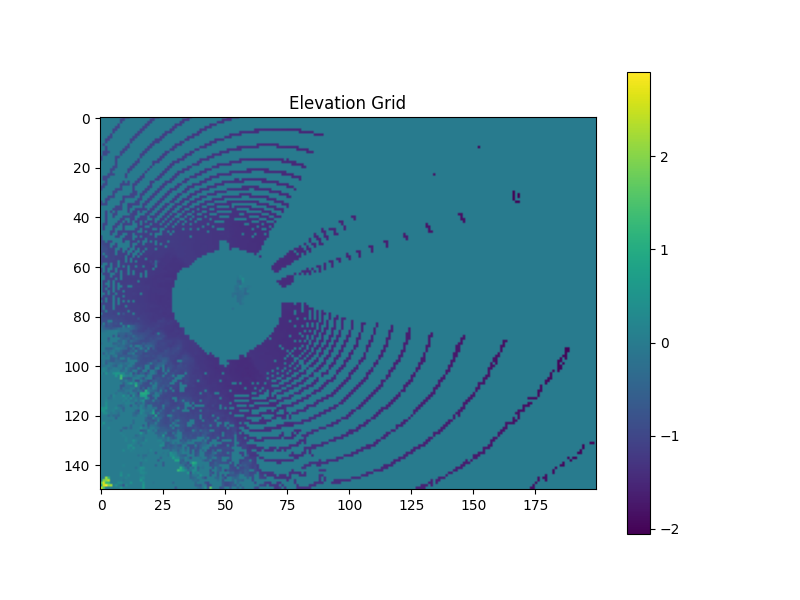
\includegraphics[width=\linewidth]{figures/rellis_elevation.png}
    \par\vspace{2pt}\footnotesize (a) Elevation Map
  \end{minipage}\hfill
  \begin{minipage}{0.31\linewidth}
    \centering
    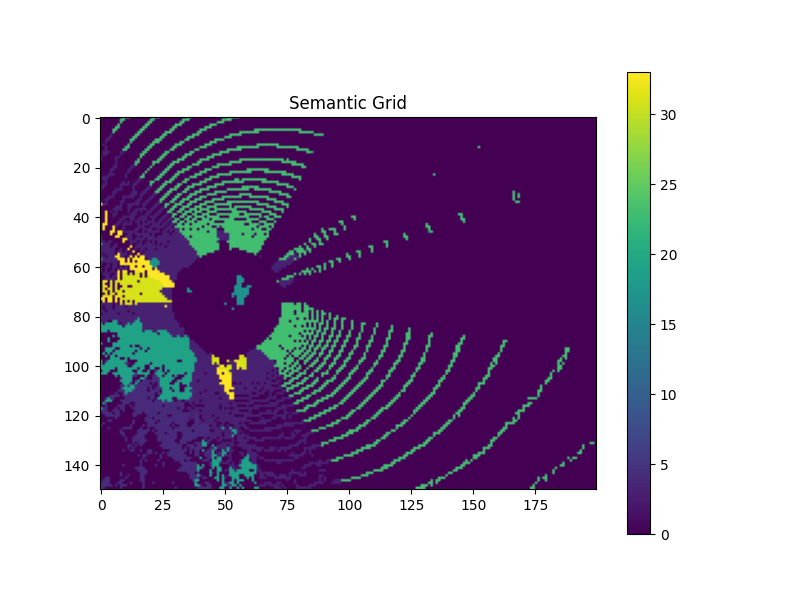
\includegraphics[width=\linewidth]{figures/rellis_semantic.png}
    \par\vspace{2pt}\footnotesize (b) Semantic Map
  \end{minipage}\hfill
  \begin{minipage}{0.31\linewidth}
    \centering
    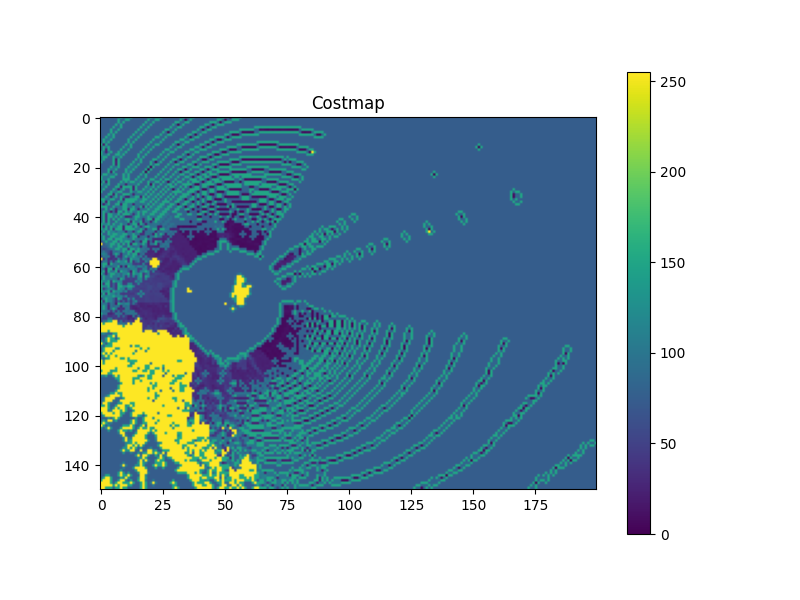
\includegraphics[width=\linewidth]{figures/rellis_costmap.png}
    \par\vspace{2pt}\footnotesize (c) Traversability Costmap
  \end{minipage}
  \caption{Multilayer 2.5D raster representations generated from raw RELLIS-3D LiDAR and semantic annotations.}
  \label{fig:rellis_maps}
\end{figure}

To validate the deployment readiness of the synthesized 2.5D dataset in robotic autonomy frameworks, we developed a dedicated ROS 2 package (\texttt{rellis\_25d\_rviz}) targeting \textbf{ROS 2 Jazzy}. The node \texttt{show\_costmap} deserializes the \texttt{.npz} files and publishes standard ROS topics:
\begin{itemize}
    \item \texttt{/costmap\_2d} (\texttt{nav\_msgs/msg/OccupancyGrid}): 2.5D traversability costmap.
    \item \texttt{/start\_marker} and \texttt{/goal\_marker} (\texttt{visualization\_msgs/msg/Marker}): Initial pose and target objective.
    \item \texttt{/astar\_path} (\texttt{nav\_msgs/msg/Path}): Reference trajectory synthesized by baseline grid A*.
\end{itemize}

\begin{figure}[htbp]
  \centering
  \begin{minipage}{0.48\linewidth}
    \centering
    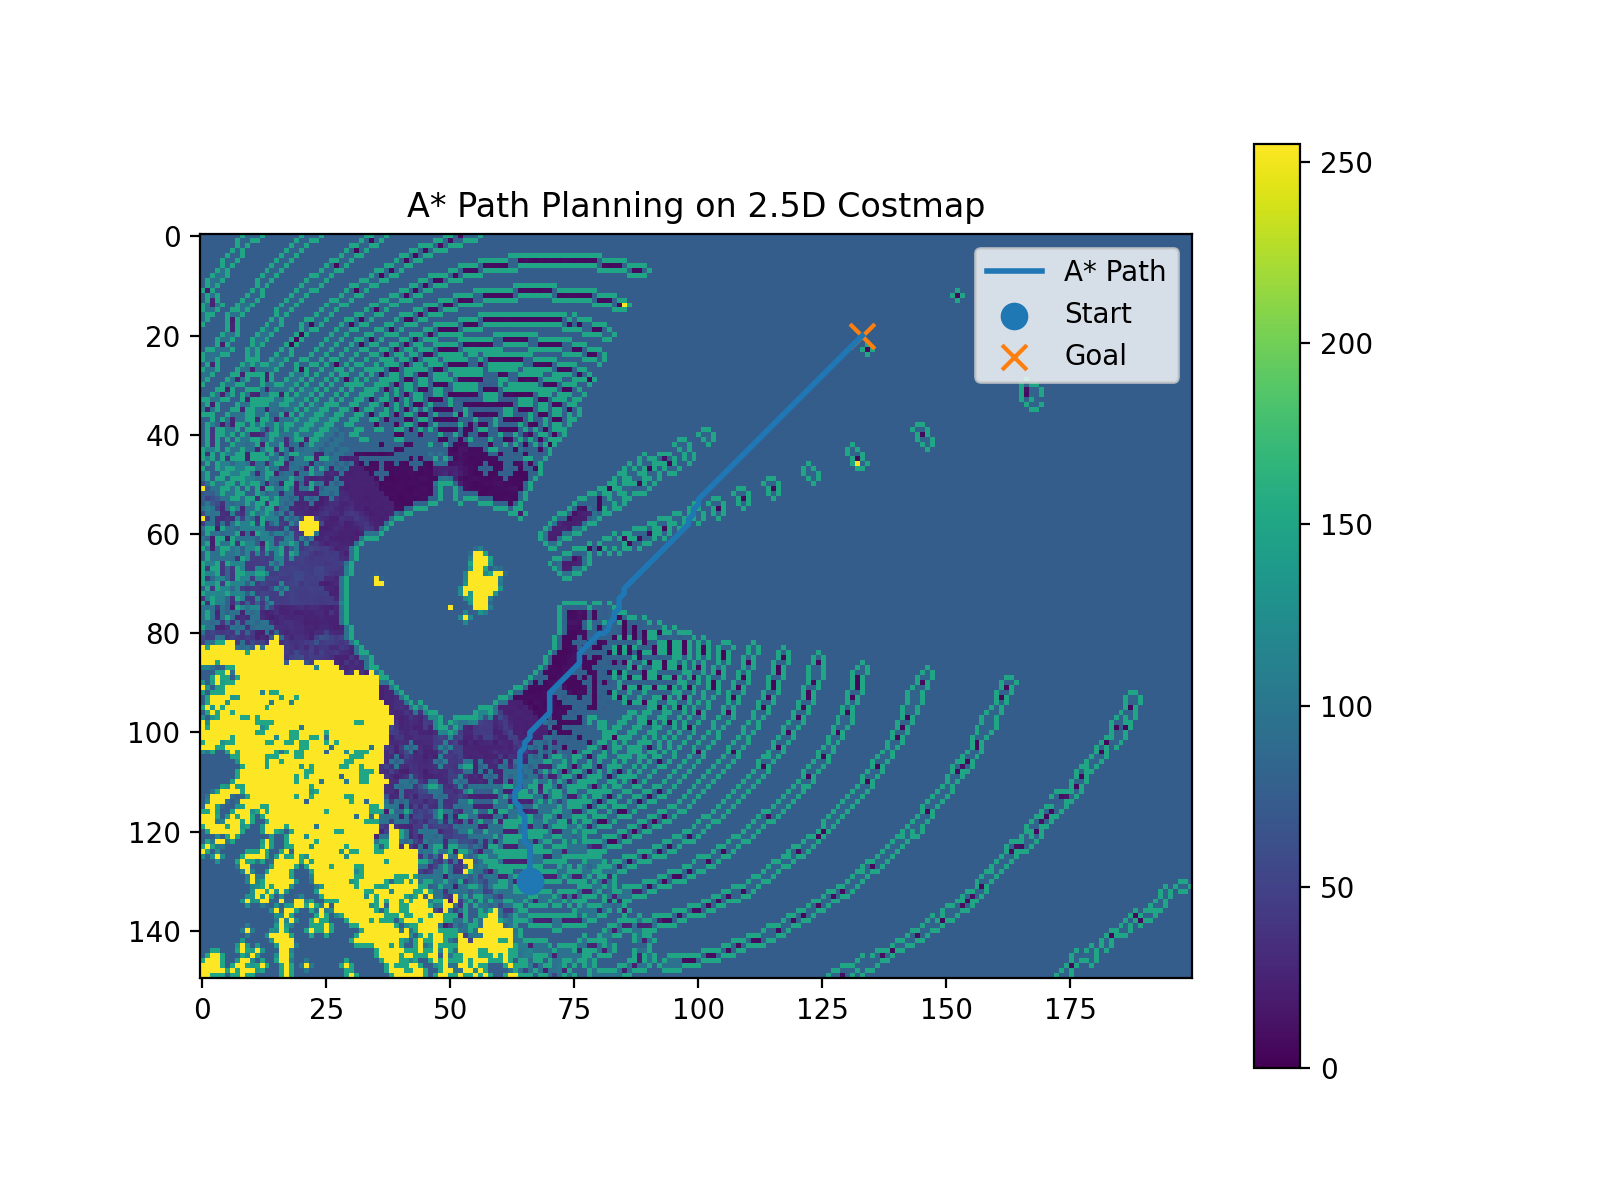
\includegraphics[width=\linewidth]{figures/rellis_astar.png}
    \par\vspace{2pt}\footnotesize (a) Planned A* path on 2.5D Costmap
  \end{minipage}\hfill
  \begin{minipage}{0.48\linewidth}
    \centering
    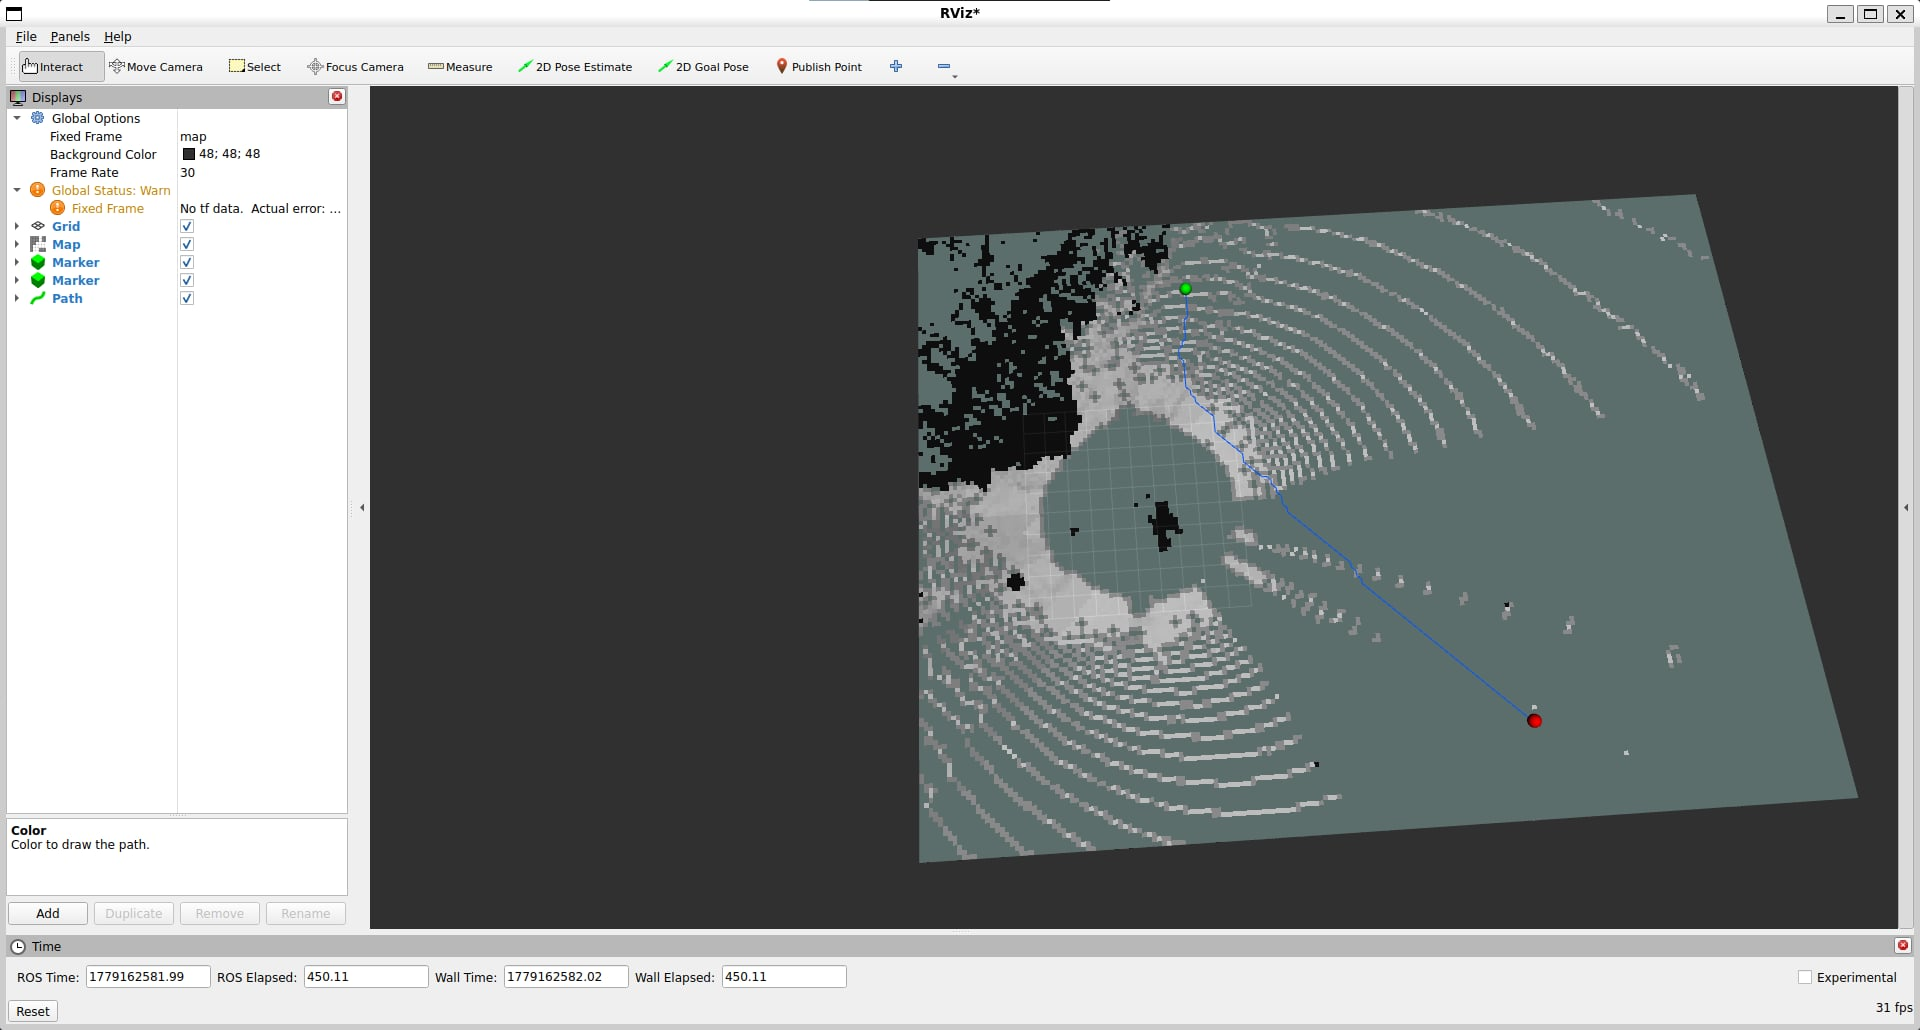
\includegraphics[width=\linewidth]{figures/rellis_rviz2.png}
    \par\vspace{2pt}\footnotesize (b) Live visualization in ROS 2 RViz2
  \end{minipage}
  \caption{Baseline A* path planning validation and real-time visualization in ROS 2 RViz2.}
  \label{fig:rviz_demo}
\end{figure}

As depicted in Fig. \ref{fig:rviz_demo}, the planning algorithm successfully routes around high-cost obstacles (trees, deep mud, fences) while selecting hard dirt and low-friction grass corridors.

\section{Theoretical Foundations of Native 2.5D Path Planning Algorithms}
\label{sec:native_theory}

While the baseline A* planner on a 2D costmap demonstrates the immediate utility of 2.5D data, it possesses inherent limitations: motion is restricted to 8 discrete grid directions, vehicle nonholonomic kinematics are neglected, and vehicle attitude dynamics (Roll/Pitch) on steep 3D terrain are not explicitly modeled.

To address these challenges, we extend our study to investigate four native 2.5D path planners designed for rough off-road terrain.

\subsection{T-Hybrid A* (Liu et al., 2023)}
\label{subsec:thybrid_astar}
T-Hybrid A* \citep{jiayangliu2023} explores a continuous 3D state space $s = (x, y, \theta)$ governed by the nonholonomic Ackermann bicycle kinematic model. The cumulative cost function $G(n)$ from the start node incorporates 3D Euclidean distance, steering angle variation, and instantaneous terrain traversability:
\begin{equation}
    G(n) = \sum_{k=1}^m \left[ \Delta L_{3D}^{(k)} + k_{\text{steer}} \cdot |\Delta \delta^{(k)}| + k_{\tau} \cdot \left(1.0 - \tau_{\text{dyn}}(s^{(k)})\right) \right]
\end{equation}
where $\Delta L_{3D} = \sqrt{\Delta x^2 + \Delta y^2 + \Delta Z^2}$, $\delta$ denotes steering angle, and $\tau_{\text{dyn}}$ is bilinearly interpolated from the 2.5D Traversability matrix.

\subsection{2.5D RRT* (Steinbauer \& Koczka, 2025)}
\label{subsec:rrt_star_25d}
2.5D RRT* \citep{geraldsteinbauer2025} expands a sample-based search tree over the continuous terrain manifold. To rigorously evaluate the kinematic feasibility of a state $(x, y, \theta)$, it projects a three-point wheel contact footprint ($P_{\text{rear}}$ at the rear axle, $P_{\text{front,left}}$ and $P_{\text{front,right}}$ at the front axle) onto the continuous elevation surface $Z$:
\begin{equation}
    \text{Roll} = \arctan\left(\frac{Z(P_{\text{fl}}) - Z(P_{\text{fr}})}{W_{\text{wheel}}}\right), \quad 
    \text{Pitch} = \arctan\left(\frac{\frac{Z(P_{\text{fl}}) + Z(P_{\text{fr}})}{2} - Z(P_{\text{r}})}{L_{\text{wheel}}}\right)
\end{equation}
The slope and attitude penalty along each branch is computed as:
\begin{equation}
    C_{\text{slope}}(n) = \left( \frac{w_{\text{roll}} \cdot |\text{Roll}|}{N} + \frac{w_{\text{pitch}} \cdot |\text{Pitch}|}{N} \right) \cdot w_{\text{slope}}
\end{equation}
Whenever $\text{Roll} > \rho_{\max}$ or $\text{Pitch} > \psi_{\max}$, the candidate edge is immediately pruned to prevent rollover.

\subsection{2.5D Field D* (Ferguson \& Stentz, 2005)}
\label{subsec:field_dstar}
2.5D Field D* \citep{fergusondavid2005} eliminates the heading discretization artifacts of conventional grid-based search by performing linear cost interpolation along cell boundaries. The synthesized path produces any-angle trajectories that continuously minimize 3D Euclidean traversal length while dynamically bypassing high-cost elevation ridges.

\subsection{2.5D LazyPRM* / ArtPlanner (Wellhausen \& Hutter, 2023)}
\label{subsec:artplanner}
ArtPlanner \citep{lorenzwellhausen2023} constructs a probabilistic manifold roadmap over the 2.5D terrain surface. Random landmark samples are efficiently connected to nearest neighbors via a \texttt{cKDTree}. The key innovation is its \textbf{Lazy Collision Checking} paradigm: the roadmap graph is evaluated first using A*, and detailed terrain edge evaluations and roll/pitch verifications are only conducted along promising path candidates, dramatically accelerating query times.

\section{Experimental Benchmarking and Dataset Quality Validation}
\label{sec:experiments}

\subsection{Experimental Setup and Evaluation Metrics}
\label{subsec:exp_setup}
Rigorous comparative benchmarks were conducted on two representative \texttt{.npz} terrain scenes:
\begin{itemize}
    \item \textbf{Map \texttt{000000.npz}:} Dimensions $40.0\text{m} \times 30.0\text{m}$ ($200 \times 150$ cells at $0.2\text{m/cell}$). Features rolling slopes, isolated mounds, and wide traversable corridors.
    \item \textbf{Map \texttt{000001.npz}:} Dimensions $40.0\text{m} \times 30.0\text{m}$. Characterized by steep ridge bands, narrow canyon corridors, and hazardous cliff edges.
\end{itemize}
The planning start position was configured at $S = (8.0\text{m}, 14.0\text{m})$ and target goal at $G = (34.0\text{m}, 25.5\text{m})$.

The quantitative evaluation suite comprises six rigorous metrics:
\begin{enumerate}
    \item \textbf{Success Rate:} Ability to find a valid, collision-free trajectory from $S$ to $G$.
    \item \textbf{Planning Time ($T_{\text{plan}}$):} Computational latency required to synthesize the trajectory (seconds).
    \item \textbf{3D Path Length ($L_{\text{3D}}$):} Actual traversed Euclidean distance in 3D space (meters).
    \item \textbf{Chassis Roll Standard Deviation ($\sigma_{\text{roll}}$):} Evaluates trajectory smoothness and ride stability ($^\circ$).
    \item \textbf{Maximum Roll Angle ($\text{Max Roll}$):} Worst-case rollover risk encountered along the route ($^\circ$).
    \item \textbf{Mean Traversability Index ($\bar{\tau}$):} Average terrain traversability score along the trajectory ($\bar{\tau} \in [0, 1]$).
\end{enumerate}

\subsection{Quantitative Benchmark Results}
\label{subsec:benchmark_results}

\begin{table}[width=\linewidth,cols=8,pos=htbp]
\caption{Quantitative performance benchmark of native 2.5D path planners on the generated terrain dataset (Extracted directly from automated test logs in \texttt{4. logs/}).}
\label{tab:benchmark_results}
\begin{tabular*}{\tblwidth}{@{} LLCCCCCC@{} }
\toprule
\textbf{Scenario} & \textbf{Algorithm} & \textbf{Success} & \textbf{$T_{\text{plan}}$ (s)} & \textbf{$L_{\text{3D}}$ (m)} & \textbf{$\sigma_{\text{roll}}$ ($^\circ$)} & \textbf{$\text{Max Roll}$ ($^\circ$)} & \textbf{$\bar{\tau}$} \\
\midrule
\multirow{4}{*}{\textbf{Map 000000}} 
& T-Hybrid A* \citep{jiayangliu2023}        & \textbf{True}  & 0.642          & 40.00          & \textbf{0.00} & \textbf{0.00}  & \textbf{1.000} \\
& 2.5D RRT* \citep{geraldsteinbauer2025}     & \textbf{True}  & 1.177          & \textbf{34.94} & \textbf{0.00} & \textbf{0.00}  & \textbf{1.000} \\
& 2.5D Field D* \citep{fergusondavid2005}   & \textbf{True}  & \textbf{0.486} & 39.75          & 2.09          & 25.10          & 0.995          \\
& 2.5D LazyPRM* \citep{lorenzwellhausen2023} & \textbf{True}  & 0.510          & 40.77          & 5.11          & 28.50          & \textbf{1.000} \\
\midrule
\multirow{4}{*}{\textbf{Map 000001}} 
& T-Hybrid A* \citep{jiayangliu2023}        & \textbf{True}  & 1.048          & 39.61          & \textbf{0.00} & \textbf{0.00}  & \textbf{1.000} \\
& 2.5D RRT* \citep{geraldsteinbauer2025}     & False          & 0.863          & 28.16          & \textbf{0.00} & \textbf{0.00}  & \textbf{1.000} \\
& 2.5D Field D* \citep{fergusondavid2005}   & \textbf{True}  & \textbf{0.461} & 39.90          & 2.86          & 25.35          & 0.992          \\
& 2.5D LazyPRM* \citep{lorenzwellhausen2023} & \textbf{True}  & 0.530          & 41.80          & 3.26          & 43.23          & 0.999          \\
\bottomrule
\end{tabular*}
\end{table}

\begin{figure}[htbp]
  \centering
  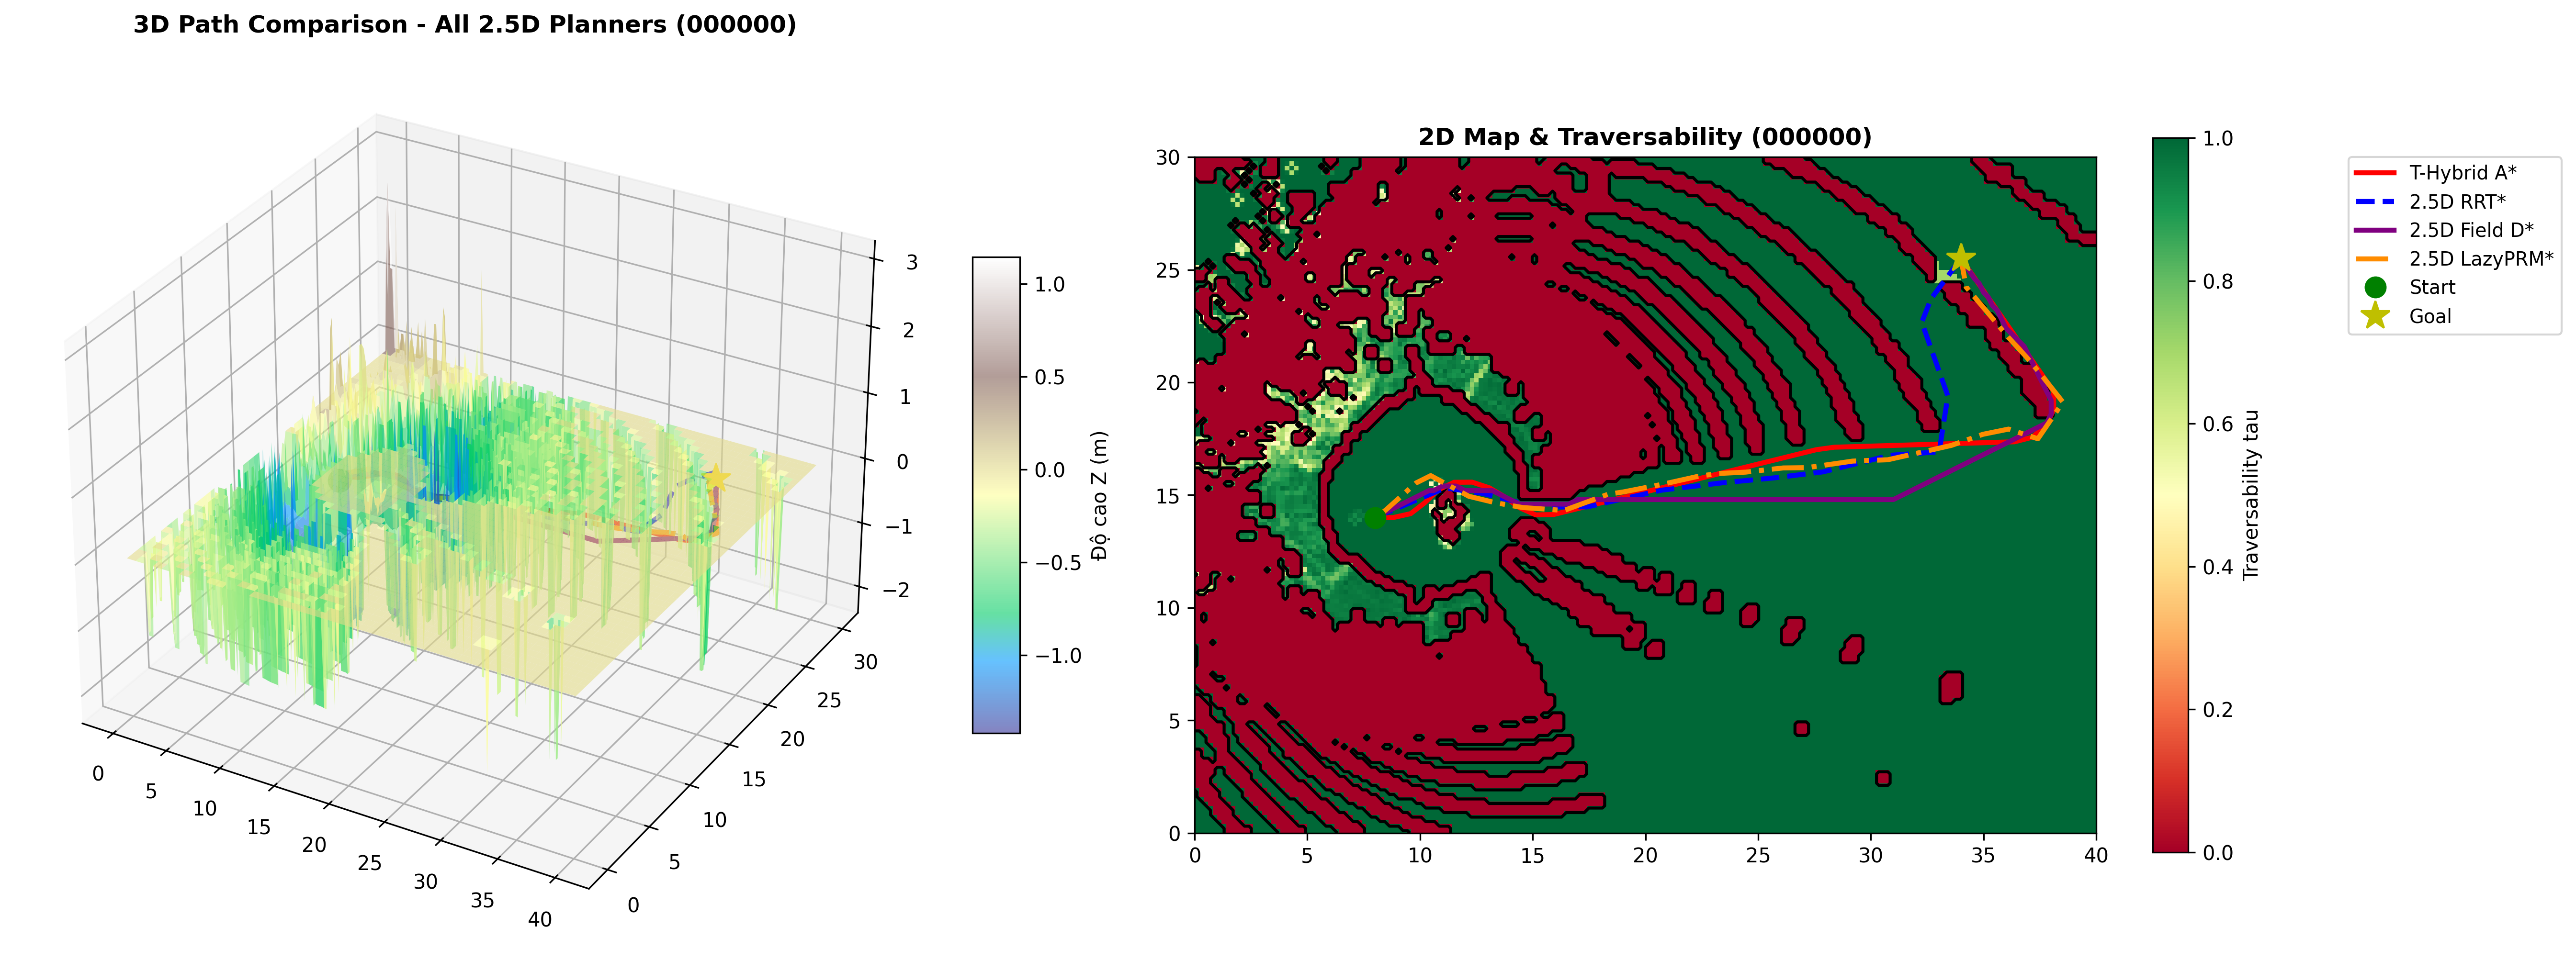
\includegraphics[width=0.92\linewidth]{figures/all_planners_000000.png}
  \caption{Visual comparison of planned 3D trajectories (left) and 2D Traversability costmaps with path corridors (right) across all four planners on Map \texttt{000000.npz}.}
  \label{fig:map_000000}
\end{figure}

\begin{figure}[htbp]
  \centering
  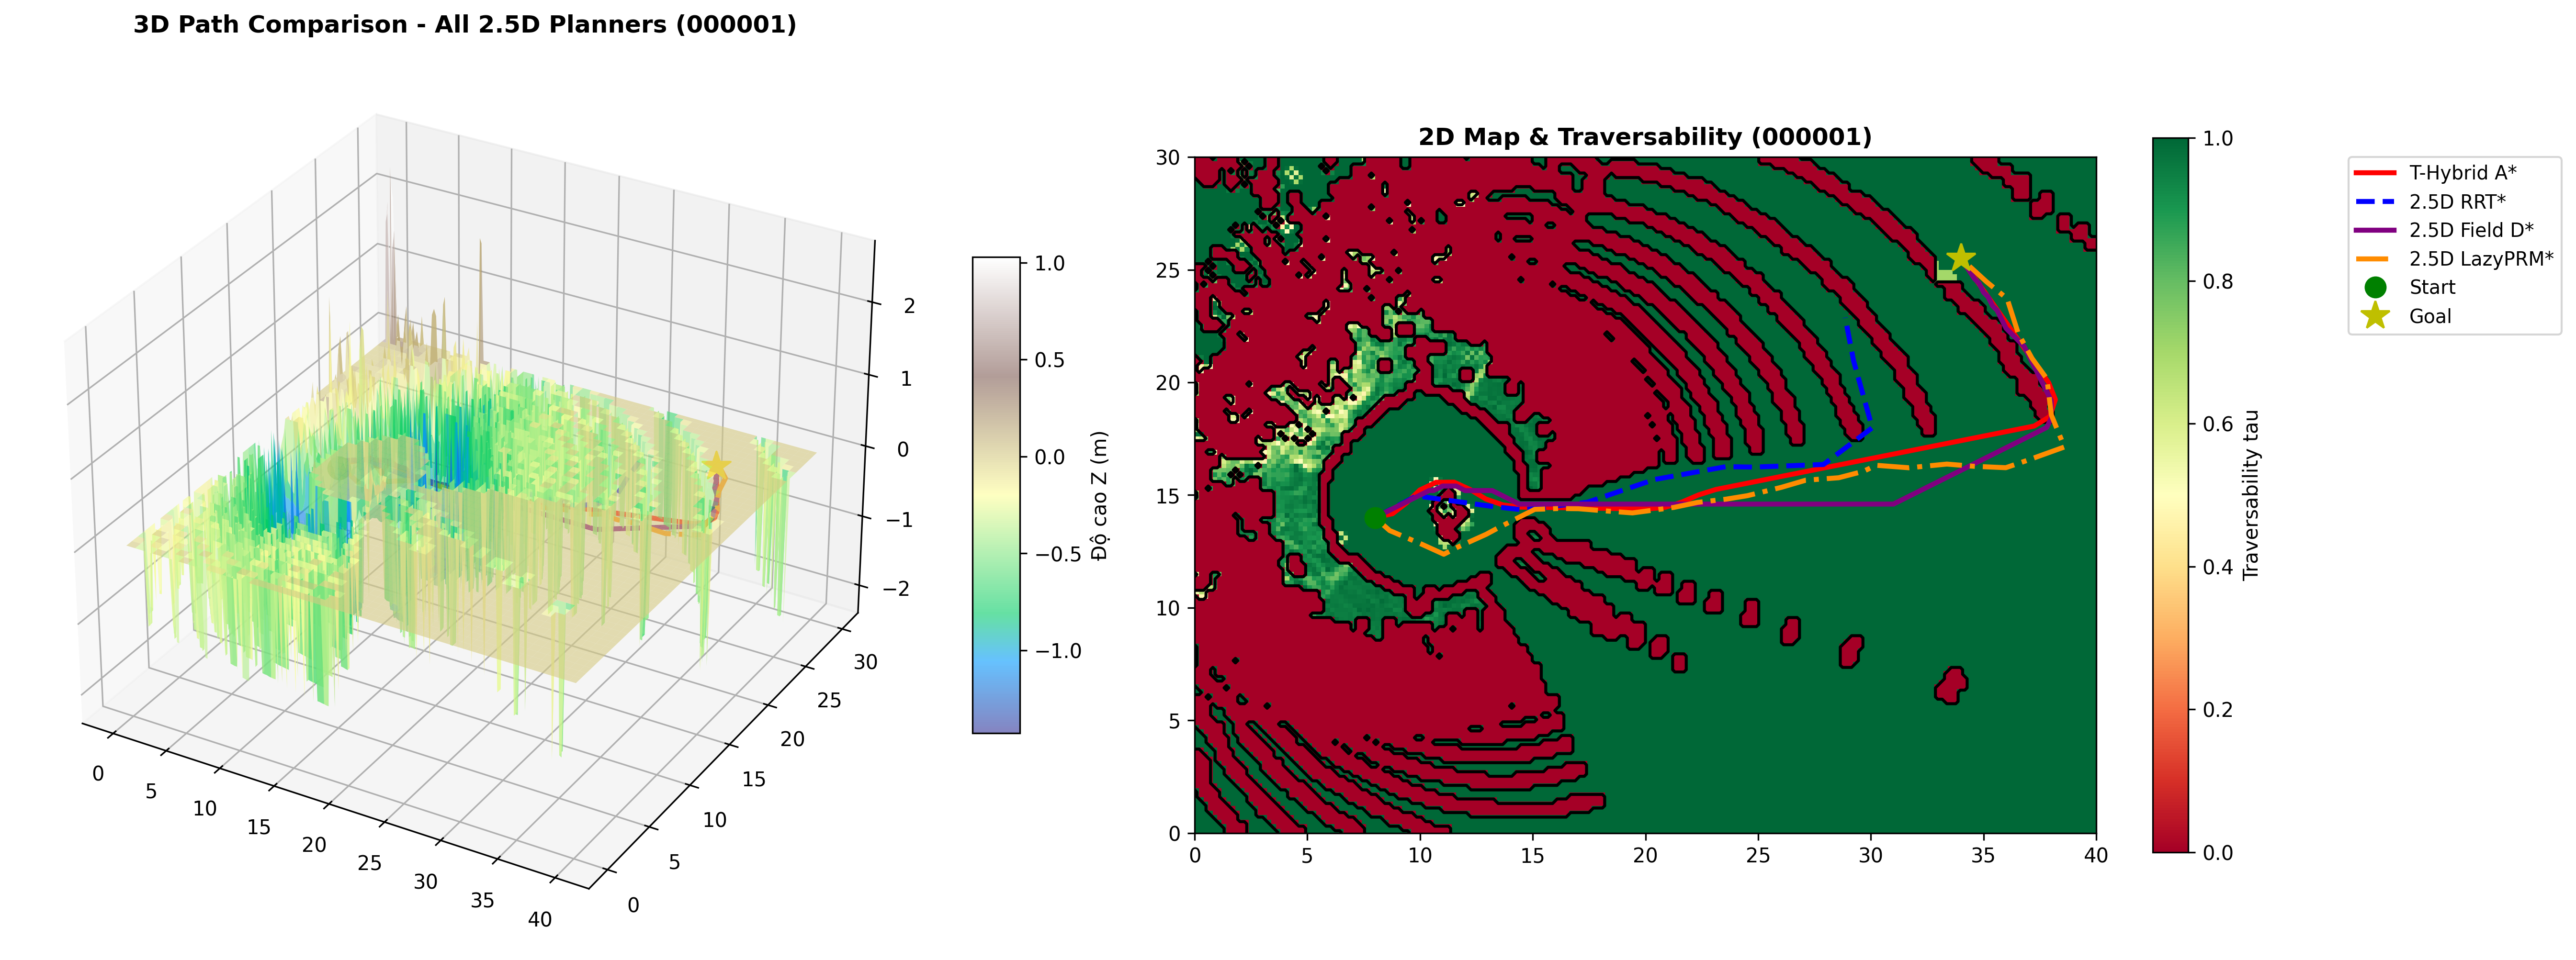
\includegraphics[width=0.92\linewidth]{figures/all_planners_000001.png}
  \caption{Visual comparison of planned 3D trajectories (left) and 2D Traversability costmaps on the steep narrow canyon topography of Map \texttt{000001.npz}.}
  \label{fig:map_000001}
\end{figure}

\subsection{Computational Efficiency and Runtime Analysis}
\label{subsec:perf_analysis}
As documented in Table \ref{tab:benchmark_results}, \textbf{2.5D Field D*} achieves the lowest computational overhead across both test scenarios ($0.461\text{s} - 0.486\text{s}$), making it exceptionally well suited for high-frequency onboard replanning. \textbf{2.5D LazyPRM*} follows closely ($0.510\text{s} - 0.530\text{s}$), demonstrating the computational advantage of its lazy collision evaluation. In contrast, \textbf{T-Hybrid A*} and \textbf{2.5D RRT*} exhibit higher latency ($0.642\text{s} - 1.177\text{s}$) attributable to numerical integration of nonholonomic dynamics and continuous footprint pitch/roll projections.

\subsection{Trajectory Quality and Vehicle Attitude Stability Analysis}
\label{subsec:stability_analysis}
\begin{itemize}
    \item \textbf{Absolute Attitude Safety:} Both \textbf{T-Hybrid A*} and \textbf{2.5D RRT*} attain a perfect traversability index $\bar{\tau} = 1.000$ and zero roll angle ($\text{Max Roll} = 0.00^\circ$). Both planners deliberately avoid cross-slope traversal, prioritizing flat and predictable ground corridors.
    \item \textbf{3D Path Length Optimization:} \textbf{2.5D Field D*} and \textbf{2.5D LazyPRM*} permit controlled chassis roll within safe bounds ($\text{Max Roll} \approx 25^\circ - 28^\circ$), effectively traversing moderate slopes to shorten 3D travel distance ($L_{\text{3D}} \approx 39.75\text{m} - 40.77\text{m}$) while maintaining high traversability scores ($\bar{\tau} \ge 0.992$).
\end{itemize}

\subsection{Adaptability to Narrow Passages and Complex Topography (Map 000001)}
\label{subsec:narrow_passage_analysis}
In Map \texttt{000001.npz}, which is constrained by steep cliffs and narrow valleys, sampling-based \textbf{2.5D RRT*} fails to reach the goal within the maximum iteration threshold (\texttt{Success = False}) due to the low probability of randomly sampling through narrow feasibility corridors. Conversely, deterministic graph-search methods (\textbf{T-Hybrid A*, Field D*, and LazyPRM*}) maintain a $100\%$ success rate, proving their superior robustness in highly constrained off-road environments.

\subsection{Evaluation of the 2.5D Terrain Dataset Quality}
\label{subsec:dataset_quality_eval}
The combined results from both phases underscore the structural integrity of the synthesized dataset:
\begin{enumerate}
    \item \textbf{Elevation Smoothness and Noise Rejection:} The 25th-percentile elevation filtering in Step 2 of Section \ref{subsec:step2_elevation} effectively eliminates spurious outliers from tall grass and overhanging canopies, yielding a continuous, $C^1$-smooth ground elevation surface $Z(x, y)$ and accurate slope derivations $\text{Slope}(x, y)$.
    \item \textbf{Fidelity of Traversability Modeling:} The composite costmap and traversability metric $\tau(x, y)$ establish clear boundaries between safe and hazardous regions. As illustrated in Figs. \ref{fig:map_000000} and \ref{fig:map_000001}, all algorithms cleanly steer clear of high-hazard red bands and converge on safe lower valleys to reach their targets.
\end{enumerate}

\section{Conclusion and Future Work}
\label{sec:conclusion}

This study has presented an end-to-end framework for digital terrain modeling and off-road motion planning:
\begin{enumerate}
    \item We developed an automated pipeline to extract multi-layer 2.5D terrain representations from RELLIS-3D into compressed \texttt{.npz} archives, seamlessly integrating geometric and semantic properties, and verified them through ROS 2 RViz2 visualization.
    \item We benchmarked four native 2.5D path planners on complex off-road terrains, validating vehicle kinematics, roll/pitch attitude stability, and traversability limits across varied topological landscapes.
\end{enumerate}

Future research will focus on incorporating dynamic soil-tire traction models (slippage, sinkage, and friction) coupled with \textbf{Model Predictive Control (MPC)} to realize robust, real-time trajectory tracking under adverse off-road conditions.

% CRediT authorship statement
\printcredits

%% Loading bibliography style file
\bibliographystyle{cas-model2-names}
\bibliography{refs}

\end{document}
